\documentclass[12pt]{article}

\usepackage{notestyle}

\graphicspath{{./img/}}


\title{Notes Software Engineering}
\author{Brendon Mendicino}



\begin{document}

\maketitle
\newpage
\tableofcontents
\newpage



\section{Introduction}
Definitions:
\begin{definition}{Multi Person Multi Version}{multi-person-multi-version}
  People coordinating in long period of time.
\end{definition}
\begin{definition}{Software}{software}
  Is a collection of code and not only digital assets like: rules, documentations, procedures and many more. 
\end{definition}
\begin{definition}{Software Types}{software-types}
  \begin{itemize}
    \item \textbf{Stand alone}: products used alone, like email, office, calendar;
    \item \textbf{Embedded in software products}: car, smart house;
    \item \textbf{Embedded in business process}: an information system;
    \item \textbf{Embedded in production process}: embedded in factories and classic production pipelines;
  \end{itemize}
\end{definition}

\subsection{Describe Software}
To describe a software we define his properties, they are divided in: \textbf{functional} property, which express an action to be performed, and \textbf{non-functional} property, that describes how a functional property should behave and describing his correctness. Because it's not possible to define if something is $100\%$ correct in the software field the \textbf{reliability} is also defined, the idea is that correctness it's impossible to obtain, thus trying to the number of \textbf{defects} a software can have, setting a threshold for the maximum number of them, on the other hand the \textbf{availability} is the percentage, over a period of time, of the system without occurring in any defect: $A = \frac{T - T_\text{down}}{T}$. Other non-functional properties are \textbf{security, safety and deniability}. \textbf{Efficiency} is the response time and the amount of resources used.

Every software has a life process divided in: development, operation, maintenance. During development, which will be the main focus of this course, there are 4 main phases:
\begin{itemize}
  \item \textbf{requirements};
  \item \textbf{design};
  \item \textbf{coding};
  \item \textbf{testing};
\end{itemize}
Basic rules of software development:
\begin{itemize}
  \item \textbf{keep it simple};
  \item \textbf{separation of concerns};
  \item \textbf{abstraction}
\end{itemize}


\subsection{Activity}
In software the base is source code, to make it more readable the code is divided in \textbf{units}, before starting to code there should be an idea of the \textbf{design} of the project, which is how and which are the units are interacting with each other. Only after the requirements and the design the coding starts. The start of the process is deciding what the software should do, those are all the \textbf{requirements}. Every part produces a result:
\begin{itemize}
  \item \textbf{Requirements} $\rightarrow$ \textbf{requirements document}
  \item \textbf{Design} $\rightarrow$ \textbf{design document}
  \item \textbf{Implementation} $\rightarrow$ \textbf{unit}
\end{itemize}
After the requirements there should be some checking with \textbf{Validation and Verification} (VV).

\subsection{Phases}
After the first version of the product is released there is a deployment phase where people will install the product, the product will need \textbf{operation} and \textbf{maintenance} operations and after a period of time the product will \textbf{retire} meaning that it will no longer be supported. During the support span the operations are all the set of the actions done on the product, like security tasting, bug discovery, etc. While maintenance is the action of changing the code to do bug fixes or publish new feature.


\section{Requirement Engineering}
The aim of requirement engineering is to define the \emph{properties of the product} before starting implementation. When defining the functionality there is one or more non-functional property associated. Requirement engineering is divided into:
\begin{itemize}
  \item \textbf{Elicitation}: talk to the end-user and understand what they want
  \item \textbf{Analysis and formalization}: writing down the 
  \item \textbf{Inspection}: checking what it has been written down on the documents
\end{itemize}
\begin{definition}{Stakeholder}{stakeholder}
  In elicitation the person in charge of the requirements has to extract all information to create the requirements, the stakeholder is the \emph{person or company} that is involved in the building of the project. The stakeholder may be: user, administrator, buyer, analyst, developer.
\end{definition}
The starting point is an informal description of the problem, usually they contain defects like: omission, inconsistencies, ambiguity. The best document is the most concise one and doesn't contain omissions, this is called \textbf{complete and consistent}.
\begin{example}{Stackeholder}{stackeholder}
  \begin{itemize}
    \item POS in a supermarket.
    \item User:
      \begin{itemize}
        \item cashier at POS (profile 1)
        \item administrator, inspector (profile 2)
        \item customer at POS
      \end{itemize}
    \item Administrator:
      \begin{itemize}
        \item POS application administrator (profile 3)
        \item IT administrator (profile 4)
        \item ...
      \end{itemize}
    \item Buyer:
      \begin{itemize}
        \item CEO of supermarket
      \end{itemize}
  \end{itemize}
\end{example}



\subsection{Context Diagram}
The context diagram tells what is the focus of the requirements. The context diagram contains the \textbf{actors} of the system which can interact with it, the system is called \textbf{use case} and there can be more than one. The context diagram defines the \textbf{interface} between the inside and outside.


\begin{example}{EZGas}{ezgas}
  \emph{"EZGas is an application to help drivers find gas at lowest prices. Gas station owners can register their gas station with prices and eventually discounts. Users look for gas stations closest to them and with best prices and quality of service."}
  
  \hfill

  \textbf{1. Stakeholder}
  \textbf{Users}: 
  \begin{itemize}
    \item Person looking for a gas station;
    \item Owner of the gas station;
    \item Workers of the gas station;
  \end{itemize}
  \textbf{Administrator}:
  \begin{itemize}
    \item App database(s) administrator;
    \item Local gas station administrator;
    \item Money transaction administrator;
  \end{itemize}
  \textbf{Buyers}: 
  \begin{itemize}
    \item Local gas station owners;
  \end{itemize}
  \textbf{2. Context diagram and interface}
  \begin{figure}[H]
    \centering
    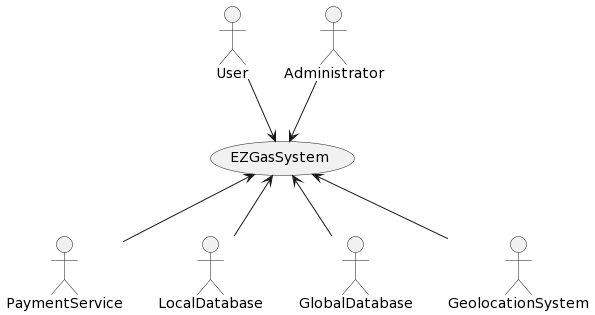
\includegraphics[width=0.8\textwidth]{context-diagram-ezgas.png}
    \caption{Context Diagram EZGas}
    \label{fig:context-diagram-ezgas}
  \end{figure}
  \begin{table}[H]
    \centering
    \begin{tabular}{|c|c|c|}
      \hline
      \textbf{Actor} & \textbf{Physical Interface} & \textbf{Logical Interface} \\
      \hline
      User & Smartphone, Internet & GUI \\
      \hline
      Administrator & Screen, Keyboard & GUI, shell \\
      \hline
      Payment System & Internet & API \\
      \hline
      Geolocation System & Internet & API \\
      \hline
      Local/Global Database & Keyboard, Internet & shell, API \\
      \hline
    \end{tabular}
    \caption{Interface Table}
  \end{table}
  \textbf{3. Functional Requirements}
  \begin{table}[H]
    \centering
    \begin{tabular}{|l|l|}
      \hline
      f1 & user authentication \\
      \hline
      f1.1 & use authentication token \\
      \hline
      f1.2 & register unregistered users \\
      \hline
      f1.3 & create new account \\
      \hline
      f2 & search gas station \\
      \hline
      f2.1 & choose search options \\
      \hline
      f2.1.1 & closest gas station \\
      \hline
      f2.1.2 & best price gas station \\
      \hline
      f2.1.3 & closest/best price mix gas station \\
      \hline
      f2.2 & select fuel kind \\
      \hline
      f2.3 & select most green company \\
      \hline
      f3 & user becoming gas station owner \\
      \hline
      f3.1 & add owned gas station \\
      \hline
      f3.1.1 & add discount \\
      \hline
      f3.1.2 & remove discount \\
      \hline
      f3.1.3 & modify gas prices \\
      \hline
      f3.1.4 & modify gas kinds \\
      \hline
      f3.2 & pay periodical fee \\
      \hline
    \end{tabular}
  \end{table}
  \textbf{5. Table of rights}
  \begin{table}[H]
    \centering
    \begin{tabular}{|l|l|l|}
      \hline
      \textbf{Actor} & \textbf{User} & \textbf{Owner} \\
      \hline
      f1 & \checkmark & \checkmark \\
      \hline
      f2 & \checkmark & \checkmark \\
      \hline
      f3 &  & \checkmark \\
      \hline
    \end{tabular}
  \end{table}
\end{example}

\hfill

\begin{example}{Robotic Vaccum Cleaner}{robotic-vaccum-cleaner}
  \emph{"Since several years robotic vacuum cleaners (RVC) are available. An RVC is capable of cleaning the floors of a house in autonomous mode. An RVC system is composed of the robot itself and a charging station. The charging station is connected to an electric socket in the house, and allows charging the battery on board of the robot. The robot itself is composed of mechanical and electric parts, a computer, and sensors. One infrared sensor in the frontal part recognizes obstacles, another infrared sensor always on the frontal part recognizes gaps (like a downhill staircase). A sensor on the battery reads the charge of the battery. The computer collects data from the sensors and controls the movement of four wheels. Another sensor on one of the wheels computes direction and distance travelled by the robot. Finally, on top of the robot there are three switches: on-off, start, learn. The learn button starts a procedure that allows the robot to map the space in the house. With a certain algorithm the robot moves in all directions, until it finds obstacles or gaps, and builds an internal map of this space. By definition the robot cannot move beyond obstacles, like walls or closed doors, and beyond gaps taller than 1 cm.  The starting point of the learn procedure must be the charging station. When the map is built the robot returns to the charging station and stops.  The start button starts a cleaning procedure. The robot, starting from the charging station, covers and cleans all the space in the house, as mapped in the ‘learn’ procedure. In all cases when the charge of the battery is below a certain threshold, the robot returns to the charging station. When recharged, the robot completes the mission, then returns to the charging station and stops."}

  \hfill
  
  \textbf{Business Model:}
  \begin{itemize}
    \item Private Company;
    \item Customers buy the RVC;
    \item Customers can bring RVC to assistance;
    \item Expert Customers can buy spare parts;
  \end{itemize}
  \textbf{1. Stakeholders:}
  \begin{itemize}
    \item Users:
      \begin{itemize}
        \item Customers;
        \item Technicians;
      \end{itemize}
    \item Administrators:
      \begin{itemize}
        \item Firmware administrator;
        \item Components administrator;
      \end{itemize}
    \item \textbf{Buyers:}
      \begin{itemize}
        \item Customer;
        \item Components Companies;
      \end{itemize}
  \end{itemize}
  \textbf{2. Context Diagram:}
  \begin{figure}[H]
    \centering
    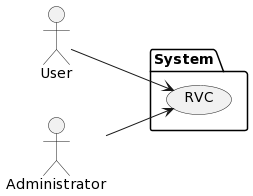
\includegraphics[width=0.3\textwidth]{rvc-context-diagram.png}
    \caption{RVC Context Diagram}
    \label{fig:rvc-context-diagram}
  \end{figure}
  \begin{table}[H]
    \centering
    \begin{tabular}{|c|c|c|}
      \hline
      \textbf{Actor} & \textbf{Physical Interface} & \textbf{Logical Interface} \\
      \hline
      Customer & Buttons & - \\
      \hline
      Administrator & Keyboard & USB \\
      \hline
    \end{tabular}
  \end{table}
  \textbf{3. Functional Properties:}
  \begin{table}[H]
    \centering
    \begin{tabular}{|l|l|}
      \hline
      f1 & perform action \\
      \hline
      f1.1 & start/stop learning \\
      \hline
      f1.2 & start/stop cleaning \\
      \hline
      f1.3 & start/stop charging \\
      \hline
      f1.4 & return to charging station \\
      \hline
      f1.5 & return to previous action \\
      \hline
      f2 & firmware update \\
      \hline
      f3 & factory reset \\
      \hline
      f4 & read data from sensors \\
      \hline
    \end{tabular}
  \end{table}
  \textbf{5. Table of Rights}
\end{example}



\section{UML}
Thanks to UML (\emph{Unified Modeling Language}) it's possible to represent the relationships between the various objects of the system. UML has many characteristics, some of which are (it the case of \emph{UML Class Diagrams}):
\begin{itemize}
  \item The Object is the \textbf{Model} of an item, every Object \emph{has unique ID}.
  \item \textbf{Class} is the descriptor of a set of items that can be grouped together.
  \item Classes can be \textbf{associated}.
  \item Every Class has \textbf{Attributes}.
\end{itemize}
In UML different class can be \emph{linked} together, this is called \textbf{Association} and represent a logical relationship between them, the association can unidirectional or bidirectional, also classes may have more than one link to represent different logical concepts. When links are formed between classes there can multiplicity of the number of classes dependent:
\begin{itemize}
  \item \texttt{1}
  \item \texttt{0..1}
  \item \texttt{0..n}
  \item \texttt{1..n}
  \item \texttt{m..n}
\end{itemize}
The \textbf{role} is how what a class represent when it has an association. This comes useful when \textbf{recursive associations} are present.

\hfill

\textbf{Composition} is indicated with a \emph{diamond}, it represent when a Class is a \emph{component} of another one, this takes a different approach with respect to inheritance, and there are two kinds:
\begin{itemize}
  \item When the diamond \textbf{is hollow} and \emph{the class A which points to B} means that, \emph{A} is part of \emph{B}.
  \item When the diamond \textbf{is full} the lifecycle are all associated, if a component dies all the other component die too.
\end{itemize}
\textbf{Generalization} is a way to implement inheritance, the parent class is pointed by a \emph{hollow arrow}. The parent class is a more generalized class, all the attributes of the generalized class are inherited by his children.


Before starting the project with UML it is import to define what are his context, e.g.:
\begin{itemize}
  \item model of concepts (glossary);
  \item model of system (system design);
  \item model of software classes;
  \item model of deployment (deployment diagram);
\end{itemize}
\emph{It's always important to minimize the number of classes.}




\subsection{Glossary}
The \textbf{glossary} or \textbf{conceptual diagram} is a way to describe the objects of our system processing. Thanks to \emph{UML Class Diagram} it's possible to represent the relationships between the various objects of the system. The glossary it's different from the \textbf{System Design}, in fact during this phase the design of the various software component must not be considered, for example the glossary representation of a university is the following:
\begin{figure}[H]
  \centering
  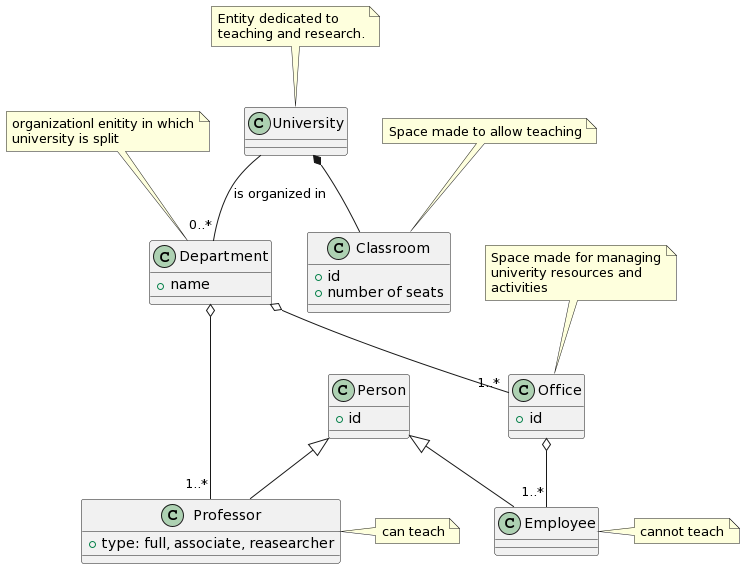
\includegraphics[width=0.8\textwidth]{university-uml-diagram.png}
  \caption{University UML Diagram}
  \label{fig:university-uml-diagram}
\end{figure}
If the name of the class is not self-explanatory a note is recommended to explain what that is or does.


\subsection{System Design}
On the other hand a \textbf{System Design} shows how the software parts of the system are related to one another, the system design can have different granularity, ranging from the representation of an entire software app reduced to a Class, to represent the real software Classes inside the application.

\subsection{UML Deployment Diagram}
The \textbf{deployment diagram} is a way to represent how the system is deployed on the physical hardware, and it uses \emph{UML Deployment Diagram}, in general every physical device is represented with a \textbf{node}, and the piece of software, library, or file that is \emph{deployed} on that physical device is called \textbf{artifact}.
\begin{figure}[H]
  \centering
  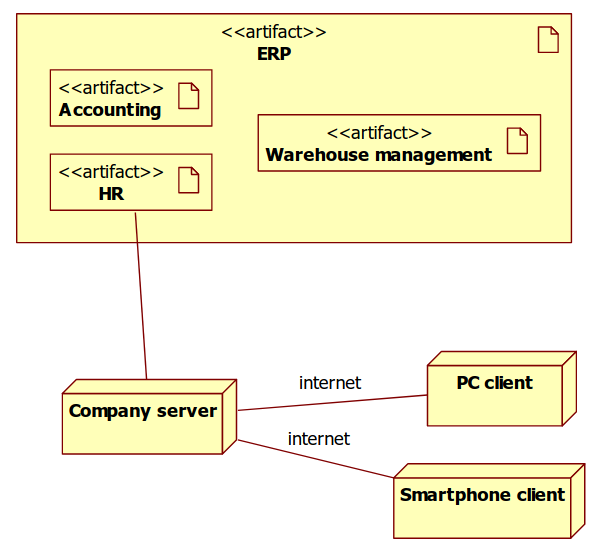
\includegraphics[width=0.6\textwidth]{deplyment-diagram-example.png}
  \caption{Deployment Diagram Example}
  \label{fig:deplyment-diagram-example}
\end{figure}

\begin{example}{Lab2 EZGas}{lab2}
  \textbf{6. Glossary}
  \begin{figure}[H]
    \centering
    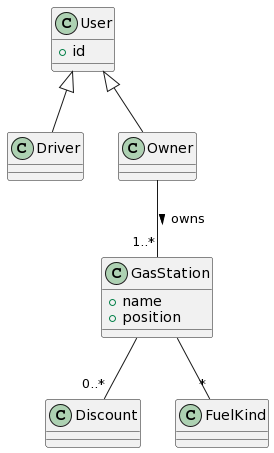
\includegraphics[width=0.4\textwidth]{ezgas-glossary.png}
    \caption{Ezgas Glossary}
    \label{fig:ezgas-glossary}
  \end{figure}
  \textbf{7. System Design}
  \begin{figure}[H]
    \centering
    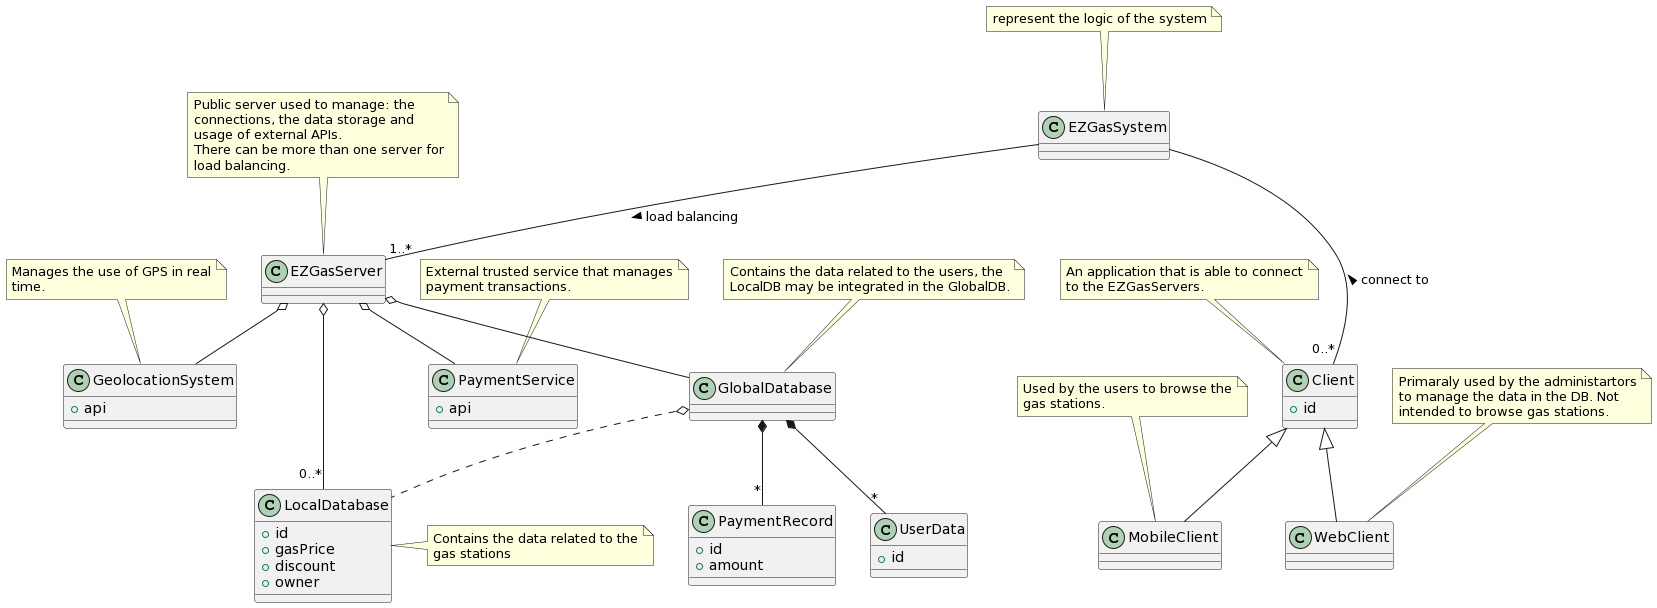
\includegraphics[width=1\textwidth]{ezgas-system-design.png}
    \caption{Ezgas System Design}
    \label{fig:ezgas-system-design}
  \end{figure}
  \textbf{8. Deployment Diagram}
  \begin{figure}[H]
    \centering
    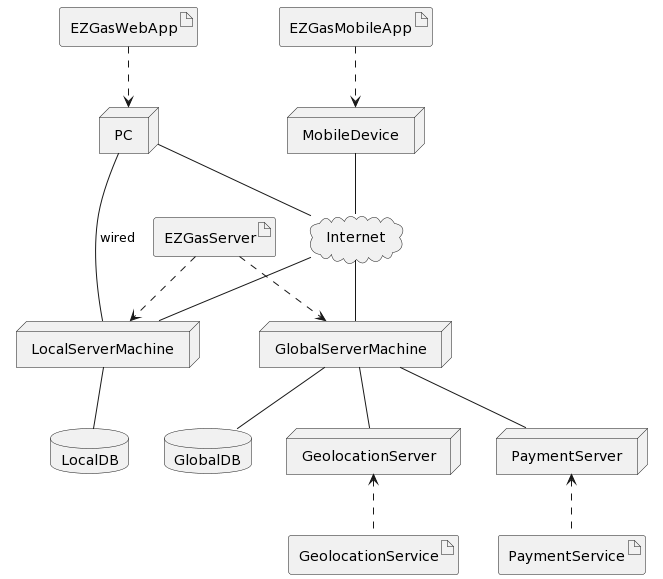
\includegraphics[width=0.8\textwidth]{ezgas-deployment-diagram.png}
    \caption{Ezgas Deployment Diagram}
    \label{fig:ezgas-deployment-diagram}
  \end{figure}
\end{example}

\hfill

\begin{example}{Lab2 RVC}{lab2-rvc}
  \textbf{6. Glossary}
  \begin{figure}[H]
    \centering
    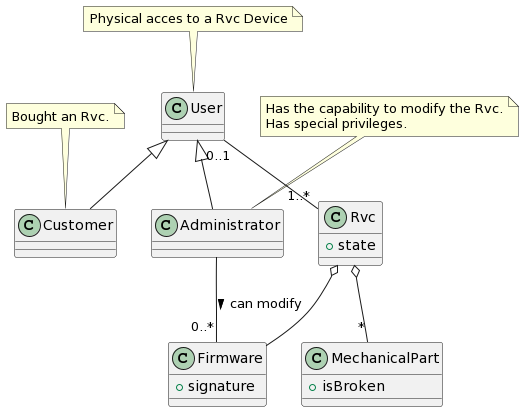
\includegraphics[width=0.6\textwidth]{rvc-glossary.png}
    \caption{Rvc Glossary}
    \label{fig:rvc-glossary}
  \end{figure}
  \textbf{7. System Diagram}
  \begin{figure}[H]
    \centering
    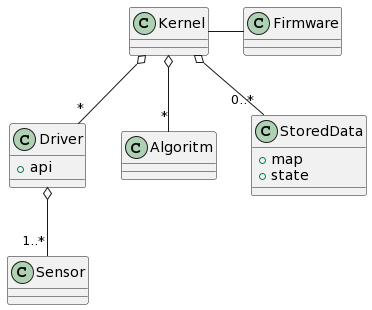
\includegraphics[width=0.4\textwidth]{rvc-system-design.png}
    \caption{Rvc System Design}
    \label{fig:rvc-system-design}
  \end{figure}
  \textbf{8. Deployment Diagram}
  \begin{figure}[H]
    \centering
    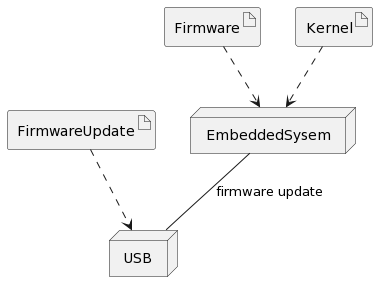
\includegraphics[width=0.4\textwidth]{rvc-deployment-diagram.png}
    \caption{Rvc Deployment Diagram}
    \label{fig:rvc-deployment-diagram}
  \end{figure}
\end{example}


\subsection{Use Cases and Scenarios}
A \textbf{scenario} is a story. To build a scenario we start from the \textbf{context diagram}, and the focus of the scenario is about explaining how the actors interact with the interfaces. Every scenario described is described with steps about what is going to happen.

On the other hand the \textbf{usecase} is the visual description of how the actor are related to the functional requirements of the system and the steps that they have to take.





\section{Non-Functional Requirements}
Non-functional requirements are some kind of properties associated to a functional property. There are some defined standard non-functional properties which are: usability, efficiency,

\textbf{Usability}: usability could be measured in:
\begin{itemize}
  \item effort to learn: to do this is experiment we can take a number of users (non-technical) and observe their responses;
\end{itemize}

\textbf{Efficiency}: represent the response time and the resource used (usually computed for the whole application, it's difficult to calculate the efficiency for a single functionality).

\textbf{Correctness}: capability of writing the right functionality, this is always unfeasible.


\textbf{Reliability}: it is the probability to encounter a defect over a period of time, the defects are bugs visible to the end-user.

\textbf{Maintainability}: is the maximum effort to operate a change on the software.

\textbf{Portability}:

\textbf{Security}: protection from malicious attacks.

\textbf{Safety}: the system is safe if it cannot harm any person or get into a hazardous situation, if it does so it needs to have some kind of control.

\textbf{Dependability}:

\subsection{EZGas}
\textbf{Scenarios and Usecases}
\begin{itemize}
  \item \textbf{Login Scenario}
    \begin{itemize}
      \item Precondition:
        \begin{itemize}
          \item User is not authenticated and not authorized;
          \item User must be registerd;
        \end{itemize}
      \item Postcondition:
        \begin{itemize}
          \item User is authenticated and authorized;
        \end{itemize}
    \end{itemize}
    \begin{enumerate}
      \item User enters the app;
      \item Inserts username and passwords;
      \item Repeat until username and passwords are correct;
      \item User is logged in;
    \end{enumerate}
  \item \textbf{Login Registration}
    \begin{itemize}
      \item Precondition:
        \begin{itemize}
          \item Download the app;
        \end{itemize}
      \item Postcondition:
        \begin{itemize}
          \item User has an account associated to a username and password;
        \end{itemize}
    \end{itemize}
    \begin{enumerate}
      \item User enters the app;
      \item Click the sign in button;
      \item Isert his username;
      \item Repeat until a valid username;
      \item Insert password;
      \item Repeat until a valid password;
      \item Insert email for password recovery;
      \item Verify email;
      \item User is now registrated;
    \end{enumerate}
  \item \textbf{User Needs Gas Station}
    \begin{itemize}
      \item Precondition: user logged in;
      \item Postcondition: user finds gas station;
    \end{itemize}
    \begin{enumerate}
      \item Users may set custom parameter for searching a gas station;
      \item User is prompted with a gas station;
      \item User may decline the gas station, if declined repeat previus step;
      \item User drives to gas station following the map instructions;
      \item User arrives;
      \item User completes his journey;
    \end{enumerate}
  \item \textbf{User Becomes GasStation Administrator}
    \begin{itemize}
      \item Precondition: user is logged in;
      \item Postcondition: user is now a gas station administrator;
    \end{itemize}
    \begin{enumerate}
      \item User wants to become a gas station owner;
      \item User enrolls to become a gas station owner;
      \item User provides his details: partita IVA;
      \item User pays monthly fee;
      \item User becomes Administrator;
    \end{enumerate}
  \item \textbf{Administrator Add GasStaion}
    \begin{itemize}
      \item Precondition: user is an administrator, administartor has acces to local/global db;
      \item Postcondition: a new gas station is added the EZGas system;
    \end{itemize}
    \begin{enumerate}
      \item Admin enters gas station owner area in the application;
      \item Admin can add or remove his owned gas stations;
      \item Admin adds all the kinds of fuel present in a gas station;
      \item Admin can add or remove discounts present for a fuel in a gas station;
      \item Changes are submitted;
      \item Validation is received from the server;
    \end{enumerate}
\end{itemize}
\begin{figure}[H]
  \centering
  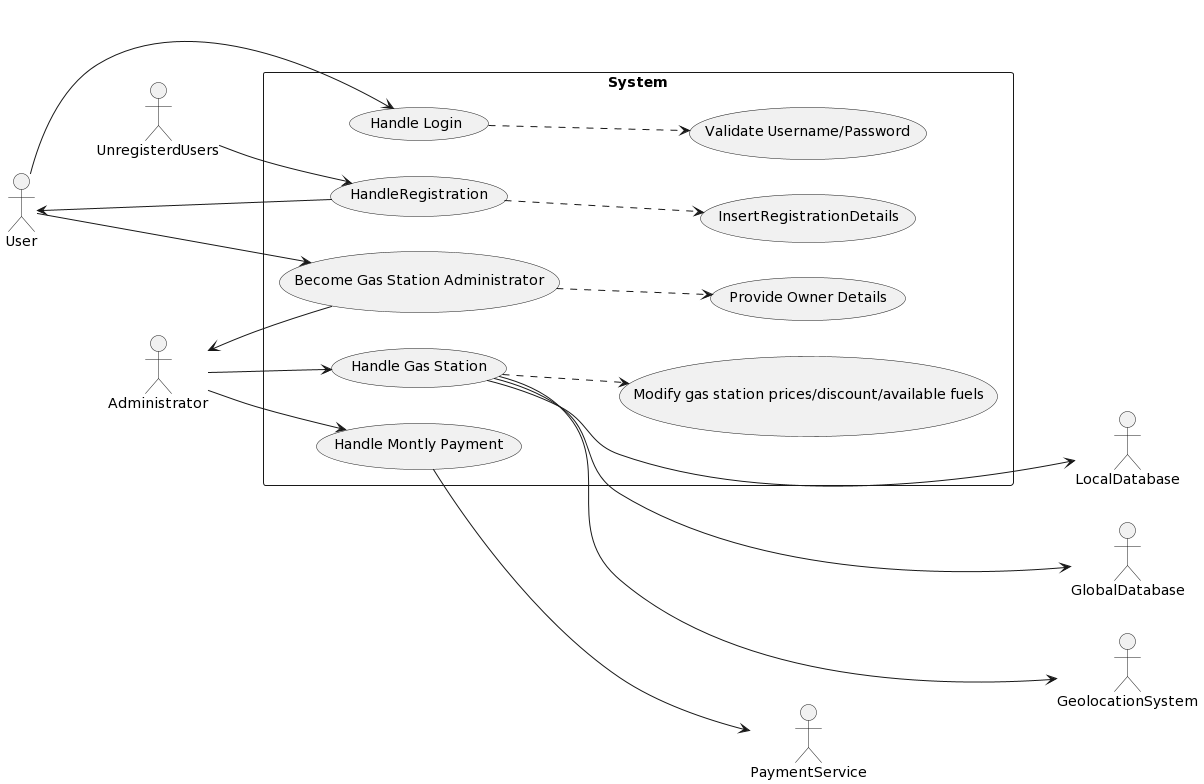
\includegraphics[width=1\textwidth]{ezgas-usecase-diagram.png}
  \caption{Ezgas Usecase Diagram, \href{http://www.plantuml.com/plantuml/uml/PP31Rjim38RlVWgXzpGlC1JTKA0Ri6B1WkvEMun3G9O2ad9X37ltIQnS9-WXWSdl9_NpVnG5rZo5Bk19dIR7D9xLUM8Sb5BiEXWqiNkDZ2E98ljNGHO7ud9ki7QiqUglVg9On0oQ3403pvX26g0kFYwYE5KuIgC7M2QCUaIUQS2ABYlwMQR24oZq84Q2xzUT8VMtR2oiw-e14CU0hZtrj-kou515to7wWB_j8ZOxTUxC7u8VKP3rMl242XJiRcA_hRfxtrKSZXJlAhQlZV-1G1uKBQK84-uF8FAMs9jwRlXgupSSqeJkkT2ZskEtYThS26BDRUp0QIQFxjTRH7RDhscJH_ti-2L53SkQkWali7pINVim4KNPD2_9qscfRfmqhnUc0MNlIOQKe-vX1WhGbqsdZCtHb4g4_yfRsUrs3pNvCxlx-mVBDhilkrtj5LvnIzJ-JRHcPhm8jZ3QXydQsM3RLb1gMscNbh_tGbhRRYi_6pUFjR0dWk-tOhmff7l4wFCK_WC0}{Link} }
  \label{fig:ezgas-usecase-diagram}
\end{figure}
\textbf{Non-Functional Requirements}
\begin{itemize}
  \item The app shall be developer for iOS, Android, Web;
  \item Avarage users should be able to learn how to use the basic functionality of the app in 10 minutes
  \item The application must satisfy the requirements of GDPR (EU) and CCPA (California) for the satisfaction of the app security.
  \item A time of 20 hour person (5 persons in a week development) to add a new feature.
  \item To develop an app for iOS, Android, Web shall take 6 months for the initial deplyment.
  \item The map must be updated once a week to avoid bringing the users into hazardous situations like: work in progress zone, accident site, ...
  \item The application server needs to have an \emph{up-time} of $99\%$ during the span of a year.
  \item The application 
\end{itemize}






\newpage
\section{Git}
Git uses distributed CMS (Content Management System) to provide version control of a project, using the concept of snapshots which allows developers to work concurrently on a single project, other than that git also has integrity with a checksum and instead of storing whole files it just stores the \textbf{delta} of the changed file (a delta represent the changes in a file based on base file). Basic git concepts:
\begin{itemize}
  \item \textbf{repository}: contains all the files and versions of the project;
  \item \textbf{working copy}: it is a snapshot of the repository, the working copy is on the client side;
  \item \textbf{commit}: it is an atomic operator that modifies the repository, all commits are tracked into a log file, to every commit a message is associated;
  \item \textbf{push}: is an operation that updates the modifications from a local server to the online server;
  \item \textbf{update}: updates the working copy by merging the changes;
  \item \textbf{staging area}: it is local dock that stores the changes that are not committed yet;
  \item \textbf{typical workflow}: checkout project, stage changes, commit;
\end{itemize}
Git basic commands: 
\begin{itemize}
  \item \texttt{\$ git init}: initialize a local repo;
  \item \texttt{\$ git remote add origin http://server.com/project.git}: add a new remote repository;
  \item \texttt{\$ git status}: status;
  \item \texttt{\$ git add}: add a file;
  \item \texttt{\$ git diff}: changes;
  \item \texttt{\$ git commit -m "..."}: commit changes;
  \item \texttt{\$ git commit -am "..."}: commit all changes;
  \item \texttt{\$ git rm}: removes a file with git tracking, adding the staging area;
  \item \texttt{\$ git mv}: moves a file adding modifications to staging area;
  \item \texttt{\$ git log}: logs;
  \item \texttt{\$ git reflog}
  \item \texttt{\$ git pull/push}
  \item \texttt{\$ git checkout <branch-name>}: switch between branches;
\end{itemize}
Every commit points to a tree which contains a list of modified files, it's possible to reach the \textbf{blob} of the changes made to that file via a pointer, every commit is linked to the previous one. The last commit of the current working branch is called \textbf{HEAD}, every HEAD points to a branch that we last commit to. If we want to switch branch we need to check out the branch, and the HEAD will change which branch it is pointing to. If there are many branches we want to bring the changes of a branch to our current one, we need to use \texttt{git checkout other-branch}, when merging two branches some \textbf{conflict} can be created, when this happens the changes need to solved by hand, in other case git is able to fix them on his own.

Other than merge there is also \textbf{rebase}, which is a bit different that merge, it tries to rewrite the history of the branch we are rebasing to and to commit all our changes to the last commit. The difference between merge and rebase, is the rebase it creates a linear commit history, while merge is keeps track of every commit where done in different branches.
\begin{itemize}
  \item \texttt{\$ git rebase -i HEAD$\sim$4}:
    \begin{itemize}
      \item -i $ \implies$ interactive mode
      \item $\sim$ 4 $ \implies$ number of commits we want to target;
    \end{itemize}
  \item \texttt{\$ git merge <other-branch>}: this command tries to merge \texttt{other-branch} inside the current working branch.
\end{itemize}
\begin{example}{Revert cahnges}{revert-cahnges}
  In case an uncommited file needs to be reset to the oringinal version it is possible to use two commands:
  \begin{itemize}
    \item \texttt{\$ git checkout <name-of-file>}
    \item \texttt{\$ git reset --hard}
  \end{itemize}
\end{example}
\begin{example}{Resolve a conflict}{resolve-a-conflict}
  When merging two branches conflicts can arise, if git is not able to automatically solve it will prompt the user to do so. When a conflict needs to be solved manually a new version of the file is created and inside both versions of the branches are present (highlighted) with conflicting sections, the conflict is solved be hand and then by committing the file.
\end{example}
\textbf{Fork and pull} is the way to go for open source development, the operation of fork copies the full project in your account and thus becoming the new owner, the two projects are separate unless it is synched to the original one.
\begin{definition}{Conventional commit message}{conventional-commit-message}
\begin{lstlisting}[language=]
<type>[optional scope]: <description>

[optional body]

[optional footer(s)]
\end{lstlisting}
  Type of commit: 
  \begin{itemize}
    \item \textbf{fix}: a commit the type \texttt{fix} patches a bug in your codebase.
    \item \textbf{feat}: a commit of type \texttt{feat} introduces a new feature to the codebase.
    \item \textbf{BREAKING CHANGE}: a commit with \texttt{BREAKING CHANGE} or appends \texttt{!}, introduces a breaking API change
  \end{itemize}
\end{definition}














\end{document}

%% vim: ts=2 sts=2 sw=2 et
